\documentclass[a4paper]{report}
\usepackage[spanish]{babel}
\selectlanguage{spanish}
\usepackage[utf8]{inputenc}
\usepackage{amssymb}
\usepackage{amsthm}
\usepackage{amsmath}
\usepackage{float}
\usepackage{blindtext}
%para incluir graficos
\usepackage{graphicx}

%para poder poner paginas en modo apaisado
\usepackage{lscape}

\usepackage{fancyhdr}

\pagestyle{fancy}
\fancyhf{}
\rhead{Año 2016}
\lhead{Proyecto Integrador}
\rfoot{Pagina \thepage}
\lfoot{Mantovani - Sambataro}

% Esto es para que el [h] me ponga las imagenes dentro de las secciones
\usepackage[section]{placeins}

\graphicspath{ {imagenes/} }



% \title{\underline{Proyecto Integrador} \\
% \huge \textbf{ \\ Plataforma concentradora de sensores y eventos digitales} \\ }
% \author{Autores: Ignacio Sambataro, Luciano Mantovani\\ \\
%   \large Tutor: PhD. Ing. Orlando Micolini \\
%   \large Supervisor: Ing. Maximiliano Eschoyez
%  % \small Facultad de Ciencias Exactas, Fisicas y Naturales\\
%  % \small Laboratorio de Arquitectura de Computadoras\\
%  % \small Universidad Nacional de Cordoba\\
%   \date{}
% }

\title{\vspace{-4cm} \textbf{Proyecto Integrador \\ \line(1,0){350}}\\
  \vspace{0.5cm}\centering{
\includegraphics[scale=0.53]{Escudo.jpg}}\\}
\author{\vspace{-0.25cm} Autores \vspace{0.25cm}\\ Luciano Mantovani - Ignacio Sambataro \bigskip \bigskip \bigskip \\
  Tema \vspace{0.25cm} \\ \textbf{ Sistema de adquisición y distribución de datos analógicos y digitales}\\ %\textbf{ Soft-Core y Soporte Linux/eCos} \\ \textbf{}
  \bigskip \bigskip \bigskip \bigskip\\
  \begin{normalsize}Director:\end{normalsize}\\
  \begin{normalsize}PhD. Orlando Micolini \end{normalsize} \\
 % \begin{normalsize}Director del Laboratorio de Arquitectura de Computadoras, FCEFyN, UNC\bigskip \bigskip \end{normalsize} \\
  \begin{normalsize}Codirector:\end{normalsize} \\
  \begin{normalsize}Ing. Maximiliano Eschoyez \end{normalsize}\\ 
 % \begin{normalsize}Integrante del Centro Universitario de Automatización y Robótica, UTN-FRC\bigskip \bigskip \end{normalsize}\\
  }
\date{}

\begin{document}
\maketitle

\clearpage

\abstract{
En este proyecto integrador se diseño y se implemento un sistema concentrador de señales de fuentes analógicas y digitales, que reúne datos y los canaliza a través de un protocolo serial hacia otro sistema que realiza distintas acciones en función de los valores de estos datos.

El concentrador es configurable vía una interfaz de linea de comando, que permite establecer, entre otras cosas, el tipo de señal de entrada que se va a recibir, el tipo de amplificación necesaria, y los intervalos de tiempo requeridos entre medición y medición, para cada entrada.

Su implementación de hardware fue hecha en base a una placa de desarrollo Silicon Labs que contiene un microcontrolador C8051F350. El software para este microcontrolador fue hecho en lenguaje C.

En una segunda etapa de este proyecto, se desarrollaron 2 implementaciones para poner en prueba el concentrador. En primera instancia, se realizo una adaptación de un sensor de campo electromagnético con su circuito electrónico. Luego, se utilizo una placa de desarrollo Raspberry Pi para implementar un sistema que interactúe con el concentrador, estableciendo una interfaz gráfica de usuario vía web, y guardando los datos que se envían y reciben en una base de datos. El software de esto ultimo fue desarrollado en Python. 
}

\clearpage

\chapter{Introducción} % (fold)
\label{cha:introduccion}

\section{Motivación} % (fold)
\label{sec:motivacion}

Este proyecto surgió de la problemática de algunos trabajos realizados dentro del Laboratorio de Arquitectura de Computadoras que compartían el mismo inconveniente. La necesidad de un sistema que genéricamente obtenga las señales de los sensores y la pueda transmitir al sistema principal, ya convertidas. Además de un contador de eventos que no requiera del uso de interrupciones por software.

Motivaciones: 

\begin{itemize}
	\item Económicas:
	    \begin{itemize}
	        \item Materiales a nuestro alcance.
	        \item Posibilidad de realizar un producto viable.
	    \end{itemize}
	\item Académicas:
	    \begin{itemize}
	        \item Oportunidad de mejorar y facilitar las mediciones de sensores analógicos y recolectar datos de señales digitales para los alumnos que realicen proyectos en el LAC (Laboratorio de Arquitectura de Computadoras). Logrando asi un concentrador generico adaptable y multiplataforma
	    \end{itemize}
	\item De Investigación:
	    \begin{itemize}
	        \item Investigar como acelerar los procesos de desarrollo de software y hardware.
	        \item Poner en uso una metodología ágil en el software.
	        \item Poner en uso una metodología ágil en el hardware.
	    \end{itemize}
	\item De Extensión:
	    \begin{itemize}
	        \item Laboratorios de Universidades de la RUNIC.
	        \item Empresas del medio.
	    \end{itemize}
	\item Tecnológicas:
	    \begin{itemize}
	        \item Utilizar tecnología madura.
	        \item Utilizar tecnología bien documentada.
	        \item Utilizas SysUML para documentar nuestro sistema
	        \item Utilizar tecnología muy difundida.
	    \end{itemize}
\end{itemize}

% section motivacion (end)

\section{Objetivos} % (fold)
\label{sec:objetivos}

\subsection{Objetivo principal} % (fold)
\label{sec:objetivo_principal}

Diseño y construcción de una placa de instrumentación de señales digitales y analógicas autónoma con un sistema de comunicación.

% section objetivos_principales (end)

\subsection{Objetivos Secundarios a Alcanzar en el Tiempo Estimado} % (fold)
\label{sec: objetivos_secundarios}

\begin{itemize}
	\item La placa debe leer entre 8 y 16 señales analógicas.
    \item La placa debe contar eventos digitales con 2 o 3 contadores distintos.
    \item La placa debe transmitir los datos digitales a través de un protocolo serial, a alguna otra placa de desarrollo o procesador.
    \item El sistema debe tener un control de ganancias programable.
    \item Lograr que el sistema tenga menor a 1,2 Vatios.
    \item Lograr que el sistema tenga la mejor inmunidad al ruido.
    \item El sistema debe ser lo mas pequeño posible.
    \item Se debe tener una sensibilidad apta para poder medir un sensor de campo electrostático.
    \item Se debe controlar el arranque y velocidad de un motor brushless con un PWM (pulse-width modulation).
    \item El sensor de campo electrostático debe tener una placa por separado para el manejo de la potencia.
    \item Se debe desarrollar un servidor web en alguna placa de desarrollo para poder controlar todas las acciones del sensor remotamente.
    \item El servidor web debe poder guardar datos de las lecturas que se realizan del sensor en una base de datos (preferentemente MySQL).
    \item Escribir la documentación sobre las instrucciones de uso para manejar el software embebido en la placa.
    \item Realizar una prueba de campo.
\end{itemize}
% section objetivos_secundarios (end)

\section{Herramientas de modelado} % (fold)
\label{sec:herramientas_de_modelado}

Para facilitar la documentación, decidimos utilizar SysUML para documentar nuestro sistema. Para esto, utilizamos la herramienta Enterprise Architect, que nos permite partir de un modelo base y reutilizar los componentes en todos los diagramas, generando vínculos que facilitan el entendimiento general del sistema. 

% section herramientas_de_modelado (end)

\section{Requerimientos} % (fold)
\label{sec:requerimientos}

\subsection{Requerimientos funcionales} % (fold)
\label{sub:requerimientos_funcionales}

Partiendo de los objetivos planteados, podemos formalizar una lista de requerimientos para nuestro sistema.

\begin{itemize}
	\item Se debería poder recibir datos de sensores analógicos en modo singular o equilibrado
	\item Se debería poder contar eventos de señales digitales cuadradas.
	\item Se debería poder configurar una ganancia especifica para canal mediante una interfaz de usuario.
	\item Se debería poder configurar un tiempo entre mediciones especifico para cada entrada mediante una interfaz de usuario.
	\item Se debería poder configurar el modo de conversión mediante una interfaz de usuario.
	\item Cada canal se debería por configurar de manera individual mediante una interfaz de usuario.
	\item El conteo de eventos, deberían ser configurables a través de una interfaz de de usuario.
	\item Se debería usar un protocolo serial para la interfaz de linea de comando entre el sistema y el usuario
	\item El usuario debería poder configurar el sistema conectándolo a un ordenador u otro sistema que soporte comunicación serial.
	\item Se debería poder enviar datos de mediciones y posibles meta-datos a través de un canal de comunicación mediante un protocolo serial.
\end{itemize}



Basandonos en los objetivos secundarios, obtenemos los siguientes requerimientos para la implementacion de un servidor web y la adaptacion para un sensor de campo electrostático:

\begin{itemize}
    \item La configuracion de los parametros para las mediciones deberian poder ser establecidas via una interfaz web grafica.
    \item Todas las interacciones del sistema deberian guardarse en una base de datos junto con un timestamp.
    \item Se deberia poder establecer un sistema de reglas que provoque que el sistema reaccione ante ciertos niveles de los datos entrantes desde el sistema de adquisicion.
    \item La placa de instrumentación desarrollada deberia poder obtener datos del sensor de campo electrostatico, proveido por profesionales de la Facultad de Matematica, Astronomia y Fisica (FaMAF).
    \item Las funcionalidades de la placa de instrumentación desarrollada deberian poder controlar el motor del sensor.
\end{itemize}

% subsection requerimientos_funcionales (end)

\subsection{Requerimientos no funcionales} % (fold)
\label{sub:requerimientos_no_funcionales}

\begin{itemize}
	\item El sistema debe documentarse con SysUML a través del programa Enterprise Architec.
	\item La plataforma de instrumentacion deberia ser portable, es decir, deberia permitir que la cantidad de sistemas embebidos compatibles sea lo mayor posible.
\end{itemize}

% subsection requerimientos_no_funcionales (end)

% section requerimientos (end)

\section{Características generales} % (fold)
\label{sec:caracteristicas_generales}

En una primera aproximación del sistema a construir, se puede establecer que se trata de un sistema capaz de recibir señales de distintos sensores digitales y analógicos. En caso que sean analógicos, convertir las señales a digital usando un conversor A-D de alta ganancia, que permita tanto entradas en modo único como como diferencial. Luego de ser convertidas, estas señales deben ser enviadas mediante un protocolo de comunicación a otro sistema que realice las acciones que deba realizar en función de los datos enviados.

En nuestro contexto interactúan 3 actores: Un usuario, uno o más sensores, y un controlador que por el momento no hacemos mención de sus características, por lo que lo llamamos simplemente ``controlador''.

\begin{figure}[h]
  \centering
  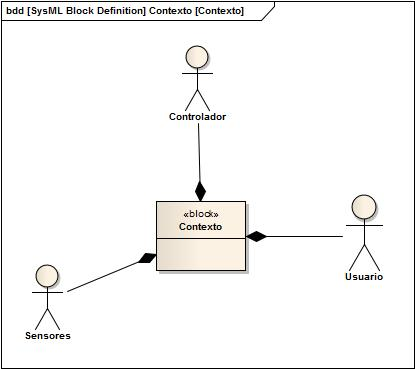
\includegraphics[width=0.80\textwidth, height = 9cm]{contexto1}
  \caption{Contexto del sistema}\label{fig:contexto1}
\end{figure}

% section caracteristicas_generales (end)

\section{Método de desarrollo} % (fold)
\label{sec:metodo_de_desarrollo}

El método de desarrollo utilizado es el desarrollo iterativo con entrega incremental. Este modelo se ilustra en la figura \ref{fig:MetodoDeDesarrollo}. En esta metodología de desarrollo el trabajo se divide en iteraciones en las cuales el producto va evolucionando. 
Un aspecto fundamental para guiar el desarrollo incremental es priorizar los requerimientos y los objetivos en función del valor que aportan al cliente. De esta manera se van añadiendo nuevos requerimientos o mejorando los que ya se completaron. Al finalizar cada iteración se obtiene un prototipo funcional.

\begin{figure}[h]
  \centering
  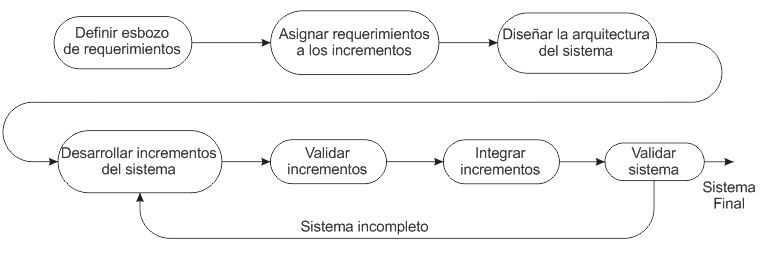
\includegraphics[width=0.80\textwidth, height = 4cm]{MetodoDeDesarrollo}
  \caption{Desarrollo incremental}\label{fig:MetodoDeDesarrollo}
\end{figure}

% section metodo_de_desarrollo (end)

\section{Casos de uso} % (fold)
\label{sec:casos_de_uso}

Dado el contexto, el sistema se puede describir de una manera general mediante un diagrama de caso de uso. El diagrama puede verse en la figura \ref{fig:casouso1}. En esta figura, se puede ver plasmados los requerimientos.

\begin{figure}[h]
  \centering
  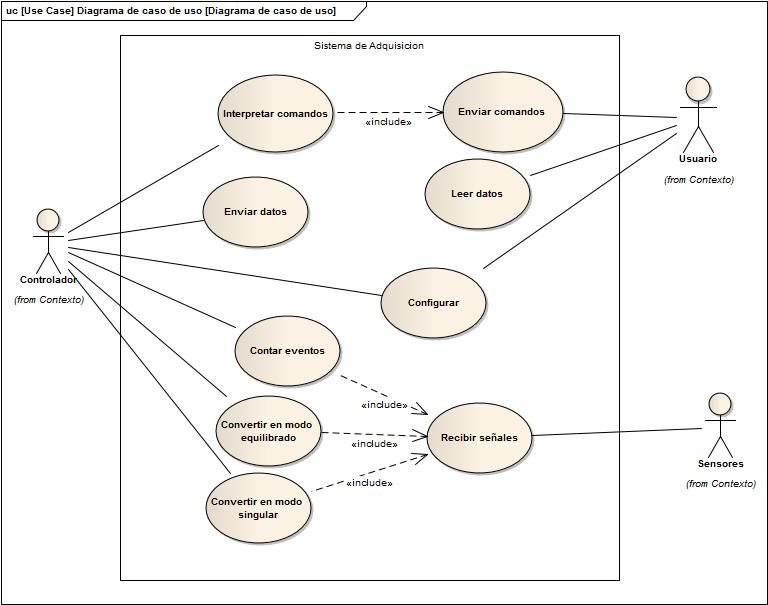
\includegraphics[width=0.80\textwidth, height = 11cm]{casouso1}
  \caption{Diagrama de caso de uso del sistema de adquisición}\label{fig:casouso1}
\end{figure}

El caso de uso ``configurar'' esta generalizado. Las acciones que incluye este caso son:
\begin{itemize}
	\item Configurar la interfaz serial
	\item Configurar canal en modo singular
	\item Configurar canal en modo equilibrado
	\item Configurar contador de eventos
	\item Configurar ganancia del del conversor
	\item Configurar intervalo de medicion para conversion analogica
\end{itemize}

% section casos_de_uso (end)

% chapter introduccion (end)


\chapter{Marco teórico} % (fold)
\label{cha:marco_teorico}


% chapter marco_teorico (end)

\chapter{Investigación} % (fold)
\label{cha:investigacion}

La etapa de investigación consistió en encontrar un microcontrolador que satisfaga la mayor cantidad de requerimientos principales. El sistema entero consiste en interactuar con el n\'ucleo, que es el microcontrolador, por lo que esta etapa requirió de análisis detallado de las opciones con las se contaba. En el cuadro \ref{tabla_micros} se pueden ver los microcontroladores considerados en la etapa de selección.

% Table generated by Excel2LaTeX from sheet 'Sheet1'
\clearpage
\begin{landscape} % TABLA DE MICROS

\begin{table}[!]
\centering
\begin{flushleft}
% Table generated by Excel2LaTeX from sheet 'Sheet1'
\scalebox{0.68}{
\begin{tabular}{|c|c|c|c|c|c|c|c|c|c|c|c|c|}
\hline
Fabricante & Modelo & RAM(K) & canales ADC & Referencia & Resolución & ganancia & Contadores & low power & puerto serie & Dimensión (') &   Pins &   Us\$ \\
\hline
 Intel & 8XC51GB &    256 &      8 &    GND & 8 bits &     no & 3 (16 bits) &     si & salida y entrada RS232 &      N &     32 &      N \\
\hline
Silicon Labs & C8051F352 &    768 &      8 & DIF/GND & 24 bits &   128x & 4 (16 bits) &     si & Smbus/$I^{2}$C, UART, SPI & 0,35x0,35 &     32 &    2,3 \\
\hline
 Atmel & AT89C5115 &    256 &      8 &    GND & 8/10 bits &     no & 3 (16 bits) &     si & UART (3 modos Full Duplex) & 0,34x0,34 &     32 &     10 \\
\hline
Microchip & PIC18F4550 &     32 &     13 &    GND & 10 bits &     no & 4(8 y 16 bits) &     si & SPI, $I^{2}$C, UART/USART, USB & 0,47x0,47 &     44 &   5,36 \\
\hline
   Nec & PD78C17 &   1024 &      8 &    GND & 8 bits &     no & 2 (8 bits) &     si & Msbus/$I^{2}$C & 0,92x0,70 &     64 &      N \\
\hline
 Maxim & DS4830 & 1024x16 &     16 & DIF/GND & 13 bits &     no & 2(16 bits) &     si & SPI, $I^{2}$C & 0,2x0,2 &     40 &    7,5 \\
\hline
   NXP & LPC1110 &      4 &      8 &    GND & 10 bits &     no & 2(32 bits) &     si & $I^{2}$C, UART, Soporte RS-485 & 0,42x0,51 &     20 &    2,5 \\
\hline
 Atmel & ATSAM3A8C &    256 &     16 & DIF/GND & 12 bits &     no & 9(32 bits) &     si & USB, SPI & 0,63x0,63 &     63 &    2,4 \\
\hline
 Atmel & ATSAM3S1A &     64 &      8 & DIF/GND & 10/12 bits & 1x,2x,4x & 3(16 bits) &     si & USB, $I^{2}$C, SPI & 0,35x0,35 &     44 &    2,5 \\
\hline
 Atmel & ATSAM3S1C &     16 &     16 & DIF/GND & 10/12 bits & 1x,2x,4x & 6(16 bits) &     si & USB, $I^{2}$C, SPI & 0,63x0,63 &     74 &    2,5 \\
\hline
 Atmel & ATSAMD21J &    256 &     20 & DIF/GND & 12 bits &    16x & 5 (16 bits) &     si & 1 USB 2.0 + 6 $I^{2}$C/USART/SPI & 0,47x0,47 &     64 &      3 \\
\hline
 Atmel & ATSAMD21G &    256 &     14 & DIF/GND & 12 bits &    16x & 3 (16 bits) &     si & 1 USB 2.0 + 6 $I^{2}$C/USART/SPI & 0,35x0,35 &     48 &    2,5 \\
\hline
 Atmel & ATSAMD21E &    256 &     10 & DIF/GND & 12 bits &    16x & 3 (16 bits) &     si & 1 USB 2.0 + 4 $I^{2}$C/USART/SPI & 0,35x0,35 &     32 &    2,5 \\
\hline
Texas Instr & MSP430F5340 &     64 &      9 &    GND & 12 bits &     2x & 7 (distintas) &     si & SPI, $I^{2}$C, UART & 0,3x0,3 &     48 &    3,3 \\
\hline
    ST & STM32F373CX &    256 &      4 &    GND & 12, 16 bits &    32x & 17 (distintas) &     si & 2 $I^{2}$C, 3 SIP, 3 USART, 1 USB & 0,35x0,35 &     48 &    2,5 \\
\hline
Atmel AVR & ATmega128 &    128 & 8 (2 c/gain) & 7 DIF, 8 GND & 10 bits & 1x, 10x, 200x & 4 (8 y 16) &     si & USART, SPI & 0,6x0,6 &     64 &      8 \\
\hline
\end{tabular}



}
\end{flushleft}
  \caption{Microcontroladores considerados}\label{tabla_micros}
\end{table}

\end{landscape}

\section{Parámetros tenidos en cuenta en la selección del microcontrolador} % (fold)
\label{sub:parametros_tenidos_en_cuenta_en_la_seleccion_del_microcontrolador}

\begin{itemize}
  \item \textbf{RAM:} No es un requisito principal, pero en caso de tener que decidir entre dos micros similares, el tamaño de la memoria puede ser un factor para tomar la decisión final
  \item \textbf{Cantidad de canales del ADC:} Mientras mas canales se tengan, mas señales analógicas de entrada pueden haber, y mas señales de sensores se podrán procesar simultáneamente
  \item \textbf{Referencia:} Nos dice si los pines del ADC se pueden usar como entrada diferencial o \'unicamente con referencia a GND. Esto es porque en el caso que haya 16 pines para el ADC y puedan usarse todos como entrada diferencial, se podrán usar como máximo la mitad de los pines, es decir 8.
  \item \textbf{Resolución:} Es la cantidad de bits con la que se representa el dato convertido. A mayor resolución, mayor presunción de la conversión.
  \item \textbf{Ganancia:} Una buena ganancia interna en el micro es necesaria para una amplificación de la señal.  evitando la mayor cantidad de ruido posible. Este parámetro es clave si se quiere trabajar con sensores que funcionan a voltajes muy pequeños en ambientes susceptibles al ruido el\'ectrico.
  \item \textbf{Contadores:} Cantidad de timers en el microcontrolador que se utilizar\'ian como contadores de eventos(es necesario que puedan ser clockeados por fuente externa, es decir, que la fuente que incrementa el contador provenga de eventos externos y no interiores al microcontrolador).
  \item \textbf{Modos de bajo consumo:} Si tiene mas de un modo de bajo consumo, es mas simple lograr que el sistema se encuentre el mayor tiempo posible consumiendo lo menor posible.
  \item \textbf{Puerto serie:} Interfaces seriales que soporta el micro. M\'inimamente se necesita que soporten $I^{2}$C y UART.
  \item \textbf{Dimensión:} Dimensión del micro. El tamaño de la placa deber\'ia ser lo menor posible por lo que mientras mas pequeño el micro, mejor.
  \item \textbf{Cantidad de pines:} Dependiendo del encapsulado, habrá una cantidad de pines. La cantidad puede afectar el tamaño y la complejidad de la placa.
  \item \textbf{Precio:} Costo en dolares del integrado.
\end{itemize}
% section parametros_tenidos_en_cuenta_en_la_seleccion_del_microcontrolador (end)

\section{Selección} % (fold)
\label{sub:seleccion}

En el momento, hab\'ia en el laboratorio una placa de desarrollo de Silicon Labs con el microcontrolador C8051F352. Este mismo fue considerado dentro de las elecciones posibles, como puede verse en el cuadro \ref{tabla_micros}.

Además de la ventaja de tenerlo en el mismo laboratorio, la placa de Silicon Labs tiene la particularidad de tener una buena ganancia máxima (128x) a la entrada del ADC, lo cual lo distingue del resto de los microcontroladores analizados. Además de esto, cumple con el resto de los requisitos propuestos por nuestro tutor, por lo que consist\'ia en una buena elección.

Habiendo hecho este análisis, se decidió optar por utilizar el microcontrolador C8051F352 de Silicon Labs.


% section selección (end)
% chapter investigacion (end)


\clearpage


\chapter{Iteración 1} % (fold)
\label{cha:iteracion_1}

% chapter iteracion_1 (end)

\chapter{Iteración 2} % (fold)
\label{cha:iteracion_2}

% chapter iteracion_2 (end)

\chapter{Sistema final} % (fold)
\label{cha:sistema_final}

% chapter sistema_final (end)



\end{document}